\section{Подготовительная часть}
	В чем заключается суть данной работы? С концептуальной стороны вопроса ответ очевиден: дан временной ряд, необходимо предсказать его следующее значение наиболее точным образом. Но прежде чем перейти к рассмотрению использованных моделей,  формализуем поставленную задачу, ведь не всегда понятно, что имеется в виду под "наиболее точно"\ и "временной ряд".
	\subsection{Формализация проблемы}
		Пусть на вход программе, назовем ее $f$, подается временной ряд вида: $y_t: t = \overline{1,N}$. Пока что никаких предпосылок относительно данного временного ряда нет. Тогда задача алгоритма $f$ предсказать $\hat{y}_{t + 1}$ так, чтобы значение $|\hat{y}_{t + 1} - y_{t + 1}|$ было минимальным. То есть $f: \mathbb{R}^{N \times 1} \to \mathbb{R} \Rightarrow f(y) = \hat{y}_{t + 1}, \text{где } y = \left(y_1,\ldots,y_N\right)^T$. В терминах глубокого обучения, имеем задачу класса sequence to one \footnote{Sequence to one - задача получения одного значения, исходя из набора данных. К таким задачам относят: семантический анализ текста, классификацию картинок и так далее.} . \textbf{Q}: Но в принципе, что такое временной ряд? \textbf{A}: Временной ряд - это последовательность значений, относящихся к одному объекту в разные моменты времени. То есть, за тот период, когда за объектом наблюдали и снимали показатели. В нашем случае временной ряд - это набор доходностей акций за определенный период времени, то есть не ставится ограничение на знак данных величин, ведь она (доходность) может быть как отрицательной, так и положительной. \textbf{Q}: Почему именно доходности? \textbf{A}: Говоря о них, нет необходимости задумываться о том, сколько реально стоит та или иная акция/ценная бумага: $20$ руб. или $2\text{'}000$ руб. В анализе доходностей нас интересует: насколько они изменяются относительно некоторого момента времени. \textbf{Q}: Какого момента? \textbf{A}: Логично представлять доходность как прирост вида:
		\begin{equation}
			r_{t} = \frac{y_{t} - y_{t - 1}}{y_{t - 1}} = \frac{y_{t}}{y_{t - 1}} - 1
		\end{equation}
		То есть, как изменяется в процентах цена на некоторый актив (не обязательно акцию, хотя в нашем случае именно на нее) относительно предыдущего рабочего дня биржи. Однако внутри самой "акции"\ фигурирует несколько показателей, характеризующих ее в конкретный момент времени: цена открытия, максимальная и минимальная цены, цена закрытия, скорректированная цена закрытия и общая сумма сделок. Акцент делается на анализе цен открытия (так как с точки зрения автора работы важнее всего - хорошо начать рабочий день), хотя несомненно наличие взаимосвязи между ценой открытия и закрытия или иными доступными показателями. Когда есть возможность - другие показатели включаются в анализ, когда нет такой возможности (классическая модель не предназначена) - не включаются. Подводя итог: \textbf{Дано}: $y = \left(y_1, \ldots, y_n\right)^T$, \textbf{Найти}: $\hat{y}_{N + 1}: |\hat{y}_{N + 1} - y_{N + 1}| \to \min$. Подставляя вышеупомянутое равенство, имеем задачу оптимизации:
		\begin{equation}
			|f(y) - y_{N + 1}| \to \min_{\beta \in \mathbb{R}^k}
		\end{equation}
		Где $\beta$ - набор параметров модели, хотя некоторые из них имеют неоптимизируемые параметры (гиперпараметры), но в общем случае задача имеет подобный вид. Но проблема в том, что $y_{N + 1}$ неизвестно, а значит, невозможно подобрать алгоритм абсолютно точного прогнозирования, значит, необходимо на основе имеющейся информации сформировать алгоритм, который наиболее точным образом описывает предложенные ему данные, а далее делает предсказание, причем предсказание, как можно меньше отличающееся от реального значения. Только теперь, проведя подобные рассуждения, мы находимся в области машинного обучения и можем говорить о гипотезах рынка \footnote{Гипотезы рынка - обоснование исследования на качественном уровне, то есть утверждения о возможности проводить какой-либо технический анализ.} . Ведь для каждого типа рынка характерны свои особенности, следовательно, закономерный вопрос: почему мы вообще имеем право пытаться предсказывать что-то для развитой или развивающейся экономик. Изложение двух нижестоящих теорий представлено в сжатом виде, что делает повествование о них поверхностным, но достаточным для понимания всех особенностей работы.
		\subsubsection{Гипотеза эффективного рынка} \label{link::hypothsis_of_msrket_efficiency}
			Это одна из самых неоднозначных в плане количества последователей инвестиционная теория, ставящая своей целью описать принципы движения цен на активы, первоначальная версия которой "представлена"\ Луи Башелье в 1900 году. В его работе показана независимость доходности акций от течения времени, таким образом, Башелье пришел к выводу: "Вероятность роста цены в любой момент времени равна вероятности ее падения, а математическое ожидание спекулянта равно нулю". Много раз менявшая свою формулировку, начиная с Пола Самуэльсона: "На конкурентных рынках на всякого продавца найдется покупатель. Если можно быть уверенным, что цена вырастет, значит, она уже выросла"\ ,  в 1960-ых годах она (гипотеза) приобрела формальный вид в труде Юджина Фамы, использовавшего в исследованиях модель случайного блуждания, выведенную Башелье. По итогам эксперимента, Юджин Фама \cite{efficient_market} привел доказательство того, что вся доступная информация уже заложена в бумагах (позднее: "рынок полностью отражает всю доступную информацию"), то есть бесполезно пытаться предугадывать цены, любое предсказание не сбудется. Более того, единственный фактор, который способен повлиять на цену - это выходящие в будущем новости. А значит, перманентное доминирование над рынком не является возможным, а активное инвестирование не является состоятельным. Более подробная информация изложена в статье от 13 сентября 2022 года \cite{fama_market_efficiency}. На данный момент существует 3 основных гипотезы эффективности рынка:
			\begin{enumerate}
				\item \textbf{Слабая гипотеза} - в цене содержится вся историческая информация об активе и только фундаментальный анализ иногда может обеспечить избыточную доходность.
				\item \textbf{Полусильная гипотеза} - в ценах содержится вся публичная информация, таким образом, избыточную доходность может обеспечить только закрытая от широкой публики информация (инсайдерская).
				\item \textbf{Сильная гипотеза} - в ценах содержится как общедоступная, так и закрытая информация. Таким образом, ничто не может дать инвесторам избыточную доходность по сравнению со среднерыночным показателем.
			\end{enumerate}
			Тогда напрашивается вывод: если быть сторонником ГЭР, то настоящая работа не имеет смысла, ведь технический анализ не может дать дополнительной доходности для любой степени ее силы. Однако, по словам Мартина Свэлла, проанализировавшего историю данной гипотезы в работе \cite{matrin_swell}: "Строго говоря, гипотеза [прежде всего, в ее сильной форме] ложна, но по духу глубоко верна $\ldots$ До тех пор, пока текущая гипотеза не будет заменена лучшей гипотезой, критика имеет ограниченную ценность". Отсюда все-таки следует обоснование, почему существует так много математических моделей, пытающихся прогнозировать доходность активов. Отсюда следует, что в современном мире количество методов предсказания настолько велико, что исследователю сложно выбрать нужный, это еще одно подтверждение, почему настоящая работа имеет смысл.
		\subsubsection{Гипотеза фрактального рынка}
			Часто в качестве доказательства ложности ГЭР приводятся в пример финансовые кризисы, так как по ГЭР вероятность возникновения подобного кризиса пренебрежимо мала или приблизительно ноль. Таким образом, появляется еще одна гипотеза: Гипотеза Фрактального Рынка (ГФР), чьим родоначальником является Бенуа Мандельброт \cite{benoit_mandelbrot}, по которой можно объяснять кризисы. Ее основные характеристики: 1) график доходностей активов имеет фрактальную (всегда $1 < D <2$) размерность 2) Различные окна (интервалы) исходного графика могут быть самоподобными 3) Каждому финансовому графику присуща своя уникальная структура и соответственно ее свойства 4) Финансовый график обладает памятью о своих исходных условиях (имеет долгосрочную память; формальный способ проверки данного утверждения вводится позже). Для выполнения данной гипотезы предполагается, что рынок является стабильным, если он включает в себе очень много инвесторов с различными горизонтами планирования (это гарантия ликвидности). Объяснение кризисов происходит следующим образом, описанным в статье Палювиной А.С. \cite{fractal_market}: "Когда инвесторы меняют свои инвестиционные горизонты (например, фундаментальная информация становится ненадёжной, а	долгосрочные инвесторы уходят с рынка или сокращают свои горизонты),	баланс между краткосрочной и долгосрочной перспективами искажается,	рынок становится менее ликвидным и возникает кризис". Таким образом, из данной гипотезы следует вывод, что информационный и инвестиционный горизонты оказывают влияние на поведение инвестора.
		\subsubsection[Проверяемая гипотеза]{Проверяемая гипотеза настоящего исследования}
			Гипотеза, подтверждение которой настоящая работа ставит одной из своих ключевых задач, заключается в проверке суждения, что нейросетевой (далее NN) поход является наиболее эффективным применительно к исследуемой области финансовых рынков, а точнее к временным рядам цен/доходностей акций. То есть главный вопрос: нейросеть лучше справляется с прогнозированием доходностей акций по цене открытия на один рабочий день биржи по сравнению с другими использованными моделями или нет?
	\subsection{Наиболее популярные методы решения}
		В настоящем исследовании последовательно рассматриваются такие модели как: Exponentially Weighted Moving Average, Auto-regressive Integrated Moving Average, Generalized Auto-Regressive Conditional Heteroskedasticity, Auto-regressive Fractionally Integrated Moving Average, Fractionally Integrated GARCH, Singular Spectrum Analysis, Fourier \& Wavelet analysis, а также Transformers и моделирование сезонности. Далее рассказывается подробнейшим образом о математической подоплеке каждой из моделей. Важно понимать, что у данной работы нет задачи предоставить полноценное обоснование, почему та или иная модель однозначно работает, однако где-то все-таки приводится подробное описание, а где-то лишь качественные рассуждения и ссылки на более подробное обоснование. Сразу стоит отметить, обращаясь к последнему пункту плана (Transformers и моделирование сезонности), что он рассматривается с точки зрения: почему он тут не нужен \cite{transformers_are_useless_for_TSF}, несмотря на революцию в Natural Language Processing, устроенную методом self-attention \cite{attention_transformers} и несмотря на важный аспект моделирования временных рядов - сезонность. Механизм self-attention создан для вычленения смысла из данных. То есть: дан набор слов, к ему в соответствие ставится вектор (она называется embedding), а после к данному набору чисел применяются известные алгоритмы ML или DL. Однако в текущей задаче в ряде доходстей или цен (одно можно получить из другого) нет контекста, то есть и сам механизм теряет свою значимость. Трансформеры оперируют понятием контекста, отвечающего за связь слова с окружающими его словами. Математически-интуитивно это можно рассматривать следующим образом: $\{w_j\}_{j=1}^n$ - все предложение, смотрим на конкретное слово (не в начале и не в конце: между словом и концом/началом должно быть как минимум еще одно слово) $w_i: i \in (1,n)$. Контекстом данного слова называется набор $w_k: k \in \{i - l, \ldots, i - 1, i + 1, \ldots, i + l\}: l \in \N$. тут пропущено само слово, так как для него окно одного размера влево и вправо является контекстом. Это значит, что при таком последовательном выборе контекста необходимо максимизировать вероятность получения конкретного слова $w_i$. Данная задача ставится в процессе создания качественного эмебддинга (сопоставления чисел словам; алгоритм Word2Vec \cite{word2vec_2013}), но в текущей задаче нет необходимости рассматривать такую смысловую взаимосвязь между величинами ряда, так как, исходя из качественных рассуждений, на вход подается единственное число, которое никак, с точки зрения смысла, не связано с другими. Исходя из этого и делается вывод, что механизм трансформеров проигрывает более простым линейным моделям \cite{transformers_are_useless_for_TSF}. Что касается сезонности, то, несмотря на подтверждение ее наличия в финансовых временных рядах \cite{seasonality_in_financial_TS_is_real}, все-таки рассматриваем модели без корректировки на данную составляющую. Подобное рассуждения приводится, опираясь на Гипотезу Эффективного Рынка, утверждающую, что финансовые временные ряды не зависят от времени, иначе рынок перестал бы быть эффективным \cite{seasonality_test_for_financial_stock_market}. Данное суждение весьма прозаично относительно показанного факта в блоке \ref{link::hypothsis_of_msrket_efficiency} о некорректности всей гипотезы в целом. В итоге получается, что из ГЭР рассматривается (принимается как верное) только суждение об отсутствии сезонности, а все остальные положения принимаются как ложные. Таким образом, в данной работе не рассматриваются как Трансформеры, так и сезонность ряда (даже если эта составляющая присутствует, то она все равно относится к шуму). Далее приступаем к описанию моделей, рассматриваемых в настоящей работе. Для удобства делим их на требующие стационарность и не требующие. \textbf{Q}: Что такое стационарность? \textbf{A}: Существует определение как для случая, когда 1) временной ряд воспринимается как последовательная реализация случайных величин как-то распределенных, так и для случая, когда 2) временной ряд - некоторый сигнал, например, от светодиода или от звукового динамика. Последовательно:
		\begin{enumerate}
			\item Временной ряд - реализация набора зависимых случайных величин с различным - изменяющимся во времени - распределением. Случайная выборка - простейший частный случай для временного ряда, так как все полученные данные являются следствием реализации не одной случайной величины с некоторым распределением, а некоторого набора. Данные распределения заранее неизвестны и их пока что не представляется физической возможности определить, так как для их определения необходимо было бы посетить параллельную вселенную, где данная величина реализовалась бы иначе. То есть для максимальной точности потребовалось бы посещения $n \to \infty$ параллельных вселенных. Отсюда и возможность оперировать только частными случаями временных рядов - случайной выборкой. Таким образом, под всеми последующими упоминаниями термина "временной ряд"\ понимается термин "случайная выборка"\ - частный случай реализации временного ряда. Для данного определения существуют 2 понятия стационарности: в узком (сильном) и в широком (слабом) смыслах. Взяты из работы  Н. В. Артамонова, Е. А. Ивина \cite{stationarity_of_time_series_econometrics}, но переработаны для удобства восприятия.
			\begin{definition} \label{def::strong_ts_stationarity}
				\textbf{Если}: $\forall p, t_1, \ldots, t_p, l \in \mathbb{N} \Rightarrow$ распределение $y_{t_1}, y_{t_2}, \ldots y_{t_p}$ идентично распределению $y_{t_1 + l}, y_{t_2 + l}, \ldots, y_{t_p + l}$. \textbf{То}: Временной ряд называется стационарным в узком смысле (строго стационарным).
			\end{definition}
			\begin{definition} \label{def::weak_ts_stationarity}
				\textbf{Если}: $\forall t \in \mathbb{N} \Rightarrow \E(y_t) = \mu \in \R, \V(y_t) = \gamma_0, \cov(y_t, y_{t - k}) = \gamma_k: \mu, \gamma_0, \gamma_k$ не зависят от $t$. \textbf{То}: Временной ряд называется стационарным в широком смысле (слабо стационарным).
			\end{definition}
 			\item Временной ряд - просто набор чисел, содержащий информацию об объекте и полученный в ходе эксперимента (наблюдения за объектом). В этом случае стационарности дается следующее определение:
 			\begin{definition} \label{def::signal_stationarity}
 				\textbf{Если}: спектр амплитуд сигнала является постоянным во времени. \textbf{То}: Сигнал называется стационарным.
 			\end{definition}
 			В данном случае имеет место деление: стационарный, значит, либо детерминированный (то есть: однозначно определяется по некоторому закону и является периодическим/квазипериодическим/непериодическим), либо случайный (например, модели финансового рынка, основанного на Броуновском Движении \cite{brownian_motion_for_stochastic_differential_equation} или Белом шуме \cite{white_noise_for_stochastic_differential_equation}); нестационарный, значит, непрерывный или переходный. Более подробно о данном понятии и формальном его осознании рассказывается в блоках \ref{link::fourier_analysis} (Анализ Фурье) и \ref{link::wavelet_analysis} (Wavelet анализ).
		\end{enumerate}
		Исходя из вышеперечисленных определений, выделяем 2 группы моделей: стационарные и нестационарные. Стационарные модели - те, для которых необходимо выполнение предпосылки о слабой (стр. \pageref{def::weak_ts_stationarity} опр. \ref{def::weak_ts_stationarity}) или сильной (стр. \pageref{def::strong_ts_stationarity} опр. \ref{def::strong_ts_stationarity}) стационарности. Нестационарные - те, для которых нет строгой необходимости в этом (они могут работать как со стационарными данными, так и с нестационарными).		
		\subsubsection{Exponentially Weighted Moving Average}
			Предполагаем, что в наличии есть данные о некотором показателе $\theta_t: t = \overline{1,n}$. В данный момент перед нами не стоит задача предсказания следующего показателя, нужно только визуально выявить тренд, чтобы приблизительно понять направление движение показателя в осях (время, значение). Конечно, в этой формулировке отсутствует строгость, пока что останавливаемся на том, что есть. Экспоненциальная скользящая средняя занимается тем, что уже заложено в ее названии: сглаживает показатели посредством усреднения. То есть в текущем значении ($t$) используется как значение в предыдущий момент времени ($t - 1$), так и значение наблюдения в момент времени ($t$). Иными словами, получается выпуклая линейная комбинация текущего и предыдущего значений:
			\begin{equation}
				v_t = \beta \cdot v_{t - 1} + (1 - \beta) \cdot \theta_t: \; \beta \in (0,1)
			\end{equation}
			Где $\beta$ - показатель, пропорциональный примерному количеству дней, по которым происходит усреднение, а $v_0 = 0$ - первое значение экспоненциальной скользящей средней. Для изучения данного рекуррентного соотношения "раскручиваем"\ его в обратном направлении:
			\begin{equation}
				\begin{split}
					v_t & =  (1 - \beta) \cdot \theta_t + \beta \cdot \overbrace{\left\{(1 - \beta) \theta_{t - 1} + \beta v_{t - 2}\right\}}^{v_{t - 1}}\\
					 & =  (1 - \beta) \cdot \theta_t + \beta \cdot \{(1 - \beta) \cdot \theta_{t - 1} + \beta \cdot \overbrace{\left\{(1 - \beta) \cdot \theta_{t - 2} + \beta \cdot v_{t - 3}\right\}}^{v_{t - 2}}\}\\
				\end{split}
			\end{equation}
			Для лучшего понимания, рассматриваем частный случае:
			\begin{equation}
				\begin{split}
					v_4 & = \beta \cdot v_3 + (1 - \beta) \cdot \theta_4\\
					v_3 & = \beta \cdot v_2 + (1 - \beta) \cdot \theta_3\\
					v_2 & = \beta \cdot v_1 + (1 - \beta) \cdot \theta_2\\
					v_1 & = \beta \cdot v_0 + (1 - \beta) \cdot \theta_1\\
					v_0 & = 0
				\end{split}
			\end{equation}
			Тогда:
			\begin{equation}
				\begin{split}
					v_4 & =  (1 - \beta) \theta_4 + \beta ((1 - \beta) \theta_3 + \beta ((1 - \beta) \theta_2 + \beta((1 - \beta) \theta_1 + \overbrace{\beta \cdot 0}^{v_0 = 0})))\\
					 & = (1 - \beta) \theta_4 + (1 - \beta) \beta \cdot \theta_3 + (1 - \beta) \beta^2 \cdot \theta_2 + (1 - \beta) \beta^3 \cdot \theta_1\\
					 & = (1 - \beta) \sum_{t = 1}^4 \beta^{4 - t} \cdot \theta_t
				\end{split}
			\end{equation}
			Аналогично происходит раскрытие и для больших показателей $v_n$. А значит, получается формула вида:
			\begin{equation}
				v_n = (1 - \beta) \sum_{t = 0}^n \beta^t \cdot \theta_{n - t}
			\end{equation}
			Отсюда качественно делаем вывод, что последним значениям наблюдаемого показателя ($\theta$) соответствует большее значение коэффициента, то есть чем ближе $\theta_{t}$ к $v_n$ с точки зрения индекса, тем больше при нем коэффициент. Теперь, возвращаясь к названию модели, отмечаем, что она должна усреднять по конкретному количеству временных единиц, следовательно, $\beta$ (единственный гиперпараметр) должен регулировать указанный показатель (то есть количество дней, по которым происходит усреднение). Обычно, рассматривается следующее соотношение: $\beta = 1 - \alpha / (N + 1)$, где $N$ - количество дней, а $\alpha$ - фактор сглаживания. Опираясь на \cite{ewma}, полагаем $\alpha = 2$ как наиболее распространенное значение.
			
			Далее рассматриваем подробнее первые значения EWMA, а конкретнее - для лучшего осознания - самое первое: $v_0 \Rightarrow v_1 = (1 - \beta) \cdot \theta_1 \Rightarrow$ при $\beta \to 1 - 0$ получаем, что $(1 - \beta) \cdot \theta_1 \ll \theta_1$, что крайне плохо отражается на самих значениях. Таким образом, вычленение тренда становится более трудным на начальных этапах из-за плохого "разогрева"\ модели. Данная проблема называет bias (смещение), а ее решение bias correction (коррекция смещения) соответственно. Основой подобной корректировки является множитель вида $(1 - \beta^t)$. Очевидно, что при $\beta \in (0,1)$, а именно так и есть по построению, $\lim\limits_{t \to +0}(1 - \beta^t) = 0$, а $\lim\limits_{t \to +\infty}(1 - \beta^t) = 1$.
			\begin{equation}
				\begin{split}
					v_n & = (1 - \beta^n)^{-1} \cdot (\beta \cdot v_{n - 1} + (1 - \beta) \cdot \theta_n)\\
					v_n & = (1 - \beta^n)^{-1} \cdot (1 - \beta) \left(\sum_{t = 0}^n \beta^t \cdot \theta_{n - t}\right)
				\end{split}
			\end{equation}
			Тогда на начальных этапах коррекция выравнивает ранее сильно уменьшенные значения EWMA, а на последующих (при $n \to \infty$) ее влияние ослабеваем, постепенно сводясь к 0 (то есть - делению на 1). Данный способ занимает очень мало памяти компьютера, так как для вычисления ему всегда необходимо хранить только 2 переменные: $v_t$ и $\beta$.
			
			Иллюстрируем вышеизложенную теорию на примере реальных данных. Рассматривается цена открытия акций компании Apple за 2021 год. Первоначально сами значения, представленные в координатах ($t$ - месяц года, $y_t$ - цена в рублях), имеют вид:
			\begin{figure}[H]
				\centering
				\begin{tikzpicture}
					\begin{axis}[
							grid = both,
							legend pos = north west,
							minor tick num = 1,
							major grid style = {lightgray},
							minor grid style = {lightgray!25},
							xlabel = {2021 год},
							width = \textwidth,
							height = 0.5 \textwidth,
							xmin=-5, xmax=260,
							ymin=115, ymax=185,
							xtick={0, 40, 80, 120, 160, 200, 240},
							xticklabels={03/01, 02/03, 28/04, 24/06, 20/08, 18/10, 14/12},
							line width=0.3mm
						]
						\addplot table [
							x=x, 
							y=Open, 
							col sep=comma,
							mark={},
							] {./source_csv/Illustration data/apple_data_test.csv};
						\legend{AAPL 2021}
					\end{axis}
				\end{tikzpicture}
				\caption{Цены открытия акций Apple (AAPL) 2021 (руб.)}
			\end{figure}
			Исходя из графика, получаем, что данные очень нестабильны, то есть с первого взгляда невозможно точно сказать, каков тренд. Однако в общих чертах графика однозначно видно, что от малых значений цен показатели переходят к б\'{о}льшим. Применяем к данным модель EWMA.
			\begin{figure}[H]
				\centering
				\begin{tikzpicture}
					\begin{axis}[
						grid = both,
						legend pos = north west,
						minor tick num = 1,
						major grid style = {lightgray},
						minor grid style = {lightgray!25},
						xlabel = {2021 год},
						width = \textwidth,
						height = 0.5 \textwidth,
						xmin=-5, xmax=260,
						ymin=115, ymax=185,
						xtick={0, 40, 80, 120, 160, 200, 240},
						xticklabels={03/01, 02/03, 28/04, 24/06, 20/08, 18/10, 14/12},
						line width=0.3mm
						]
						\addplot table [
						x=x, 
						y=Open, 
						col sep=comma,
						mark={},
						] {./source_csv/Illustration data/apple_data_test_ewma.csv};
						%\legend{AAPL 2021};
						
						\addplot table [
						x=x, 
						y=V_2, 
						col sep=comma,
						mark={},
						] {./source_csv/Illustration data/apple_data_test_ewma.csv};
						%\legend{EWMA $\beta = 0.1$};
						
						
						\addplot table [
						x=x, 
						y=V_10, 
						col sep=comma,
						mark={},
						] {./source_csv/Illustration data/apple_data_test_ewma.csv};
						%\legend{EWMA $\beta = 0.1$};
						
						\addplot table [
						x=x, 
						y=V_30, 
						col sep=comma,
						mark={},
						] {./source_csv/Illustration data/apple_data_test_ewma.csv};
						%\legend{EWMA $\beta = 0.3$};
						
						\addplot table [
						x=x, 
						y=V_50, 
						col sep=comma,
						mark={},
						] {./source_csv/Illustration data/apple_data_test_ewma.csv};
						%\legend{EWMA $\beta = 0.5$};
						
						
						\addplot table [
						x=x, 
						y=V_90, 
						col sep=comma,
						mark={},
						] {./source_csv/Illustration data/apple_data_test_ewma.csv};
						%\legend{EWMA $\beta = 0.9$};
						
						\addplot table [
						x=x, 
						y=V_200, 
						col sep=comma,
						mark={},
						] {./source_csv/Illustration data/apple_data_test_ewma.csv};
						%\legend{EWMA $\beta = 0.9$};
						
						\legend{AAPL 2021, $n = 2$, $n = 10$, $n = 30$, $n = 50$, $n = 90$, $n = 200$};
					\end{axis}
				\end{tikzpicture}
				\caption{EWMA, цены открытия AAPL 2021 (руб.)}
			\end{figure}
			Глядя на полученный результат сразу ясно, что тренд восходящий, однако это предположение делается только на основе визуального анализа. Пока что никаких алгоритмов нет. Однако нельзя недооценивать полученную информацию, так как более явный тренд позволяет моделям (нейронных сетей) более точно настраиваться на обучающую выборку, что часто приводит к улучшению результату предсказаний (если, конечно не довести до переобучения: данные термины и теория объясняется в блоке \ref{link::neural_networks} стр. \pageref{link::neural_networks}). Также стоит отметить всплеск, случившийся при $n = 2$. Это произошло именно именно из-за технических особенностей добавленного множителя, корректирующего смещение. 
			
			Последним пунктом необходимо рассказать более подробно о самом корректирующем множителе. \textbf{Q}: Почему у него именно такой вид, ведь можно просто сделать первое значение таким же, как в исходном ряде? \textbf{A}: 1) необходимо корректировать вычисления, исходя из одной формулы, так как цель - прийти именно к общности 2) при последующих наблюдения данный коэффициент становится чрезвычайно малым $\lim\limits_{t \to +\infty}(1 - \beta^t) = 1$, а при первоначальных значениях не оказывает влияния $\lim\limits_{t \to +0}(1 - \beta^t) = 0$. Однако при индексах (речь о непрерывных), стремящихся к $0$, обратная величина стремится к $\infty$, что очень плохо с вычислительной точки зрения, так как у компьютера может произойти переполнение памяти и вместо числа получится NaN или Null, что не позволит далее осуществлять расчеты. Поэтому в начале графике наблюдается резкий всплеск, сходящийся впоследствии к исходному ряду. Далее приводится график значений корректирующих коэффициентов в зависимости от $\beta$ и от $t$.
			\begin{figure}[H]
				\centering
				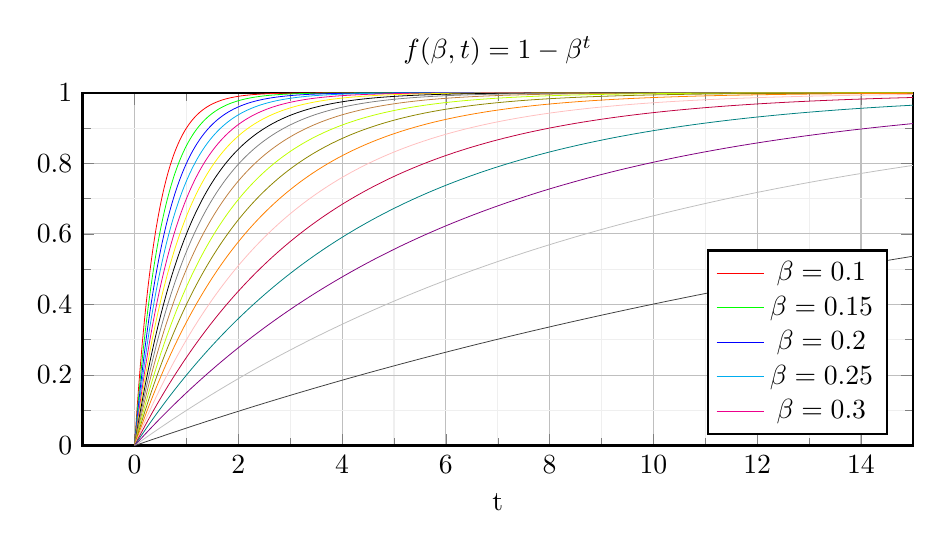
\begin{tikzpicture}
					\begin{axis}[
						grid = both,
						legend pos = south east,
						minor tick num = 1,
						major grid style = {lightgray},
						minor grid style = {lightgray!25},
						title={$f(\beta, t) = 1 - \beta^t$},
						xlabel = {t},
						width = \textwidth,
						height = 0.5 \textwidth,
						xmin=-1, xmax=15,
						ymin=0, ymax=1,
						%xtick={0, 40, 80, 120, 160, 200, 240},
						%xticklabels={03/01, 02/03, 28/04, 24/06, 20/08, 18/10, 14/12},
						line width=0.3mm
						]
						\addplot[domain = 0:15,
						samples = 300,
						color = red,
						smooth,
						line width = 0.01cm,] {1 - 0.1^x};
						\addplot[domain = 0:15,
						samples = 300,
						color = green,
						smooth,
						line width = 0.01cm,] {1 - 0.15^x};
						\addplot[domain = 0:15,
						samples = 300,
						color = blue,
						smooth,
						line width = 0.01cm,] {1 - 0.2^x};
						\addplot[domain = 0:15,
						samples = 300,
						color = cyan,
						smooth,
						line width = 0.01cm,] {1 - 0.25^x};
						\addplot[domain = 0:15,
						samples = 300,
						color = magenta,
						smooth,
						line width = 0.01cm,] {1 - 0.3^x};
						\addplot[domain = 0:15,
						samples = 300,
						color = yellow,
						smooth,
						line width = 0.01cm,] {1 - 0.35^x};
						\addplot[domain = 0:15,
						samples = 300,
						color = black,
						smooth,
						line width = 0.01cm,] {1 - 0.4^x};
						\addplot[domain = 0:15,
						samples = 300,
						color = gray,
						smooth,
						line width = 0.01cm,] {1 - 0.45^x};
						\addplot[domain = 0:15,
						samples = 300,
						color = brown,
						smooth,
						line width = 0.01cm,] {1 - 0.5^x};
						\addplot[domain = 0:15,
						samples = 300,
						color = lime,
						smooth,
						line width = 0.01cm,] {1 - 0.55^x};
						\addplot[domain = 0:15,
						samples = 300,
						color = olive,
						smooth,
						line width = 0.01cm,] {1 - 0.6^x};
						\addplot[domain = 0:15,
						samples = 300,
						color = orange,
						smooth,
						line width = 0.01cm,] {1 - 0.65^x};
						\addplot[domain = 0:15,
						samples = 300,
						color = pink,
						smooth,
						line width = 0.01cm,] {1 - 0.7^x};
						\addplot[domain = 0:15,
						samples = 300,
						color = purple,
						smooth,
						line width = 0.01cm,] {1 - 0.75^x};
						\addplot[domain = 0:15,
						samples = 300,
						color = teal,
						smooth,
						line width = 0.01cm,] {1 - 0.8^x};
						\addplot[domain = 0:15,
						samples = 300,
						color = violet,
						smooth,
						line width = 0.01cm,] {1 - 0.85^x};
						\addplot[domain = 0:15,
						samples = 300,
						color = lightgray,
						smooth,
						line width = 0.01cm,] {1 - 0.9^x};
						\addplot[domain = 0:15,
						samples = 300,
						color = darkgray,
						smooth,
						line width = 0.01cm,] {1 - 0.95^x};
						\legend{$\beta = 0.1$, $\beta = 0.15$, $\beta = 0.2$, $\beta = 0.25$, $\beta = 0.3$};
					\end{axis}
				\end{tikzpicture}
				\caption{График корректирующих коэффициентов}
			\end{figure}
			В трехмерном пространстве это выглядит так:
			\begin{figure}[H]
				\centering
				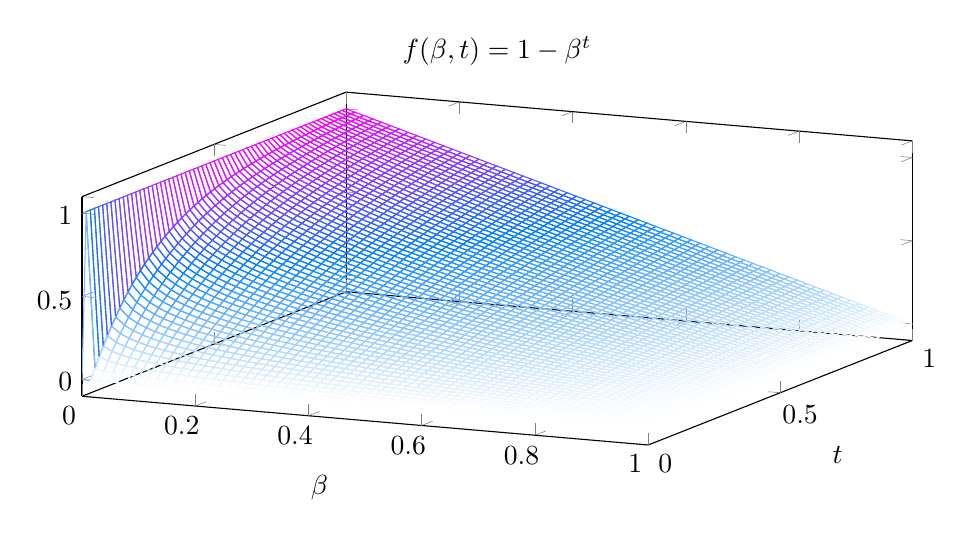
\begin{tikzpicture}
					\begin{axis}
						[
						title={$f(\beta, t) = 1 - \beta^t$},
						%hide axis,
						colormap/cool,
						width = \textwidth,
						height = 0.5 \textwidth,
						xlabel={$\beta$},
						ylabel={$t$}
						] 
						\addplot3[
						mesh,
						samples=65,
						domain=0:1,
						]{1 - x^y};
					\end{axis}
				\end{tikzpicture}
				\caption{Трехмерное изображение корректирующих коэффициентов}
			\end{figure}
			Данная модель является наиболее простой, однако она обладает возможностью предсказания.
			\begin{equation}
				\begin{split}
					v_{t + 1} & = k \cdot y_t + (1 - k) \cdot v_t: \; k \in (0, 1)
				\end{split}
			\end{equation}
			В данном случае $v_t$ - это предсказанное значение на момент времени $t$. Модель не является устойчивой к наличию сезонности и тренду, однако факт того, что предсказания возможны есть. Значит, эта модель включается в список попадающих в сравнительную таблицу.
		\subsubsection{Auto-regressive Integrated Moving Average}
		\subsubsection{Generalized Auto-Regressive Conditional Heteroskedasticity}
		\subsubsection{Auto-regressive Fractionally Integrated Moving Average}
		\subsubsection{Fractionally Integrated GARCH}
		\subsubsection{Singular Spectrum Analysis}
		\subsubsection{Fourier analysis} \label{link::fourier_analysis}
		\subsubsection{Wavelet analysis} \label{link::wavelet_analysis}
		\subsubsection{Neural Networks} \label{link::neural_networks}
			\subsubsubsection{Multilayer Perceptron}
			\subsubsubsection{Recurrent Neural Network}
			\subsubsubsection{Wavelet Network}
			\subsubsubsection{Алгоритмы обучения: GD семейство}
			
